\documentclass[12pt]{article}

\usepackage[dvips,letterpaper,margin=0.75in,bottom=0.5in]{geometry}
\usepackage{cite}
\usepackage{slashed}
\usepackage{graphicx}
\usepackage{amsmath}
\usepackage{braket}

\usepackage[american,fulldiode]{circuitikz}
\usetikzlibrary{calc}

\newcommand{\kb}{k_{\rm b}}
\begin{document}
\ctikzset{bipoles/thickness=1}
\ctikzset{bipoles/resistor/height=.115}
\ctikzset{bipoles/resistor/width=.3}
\ctikzset{bipoles/capacitor/height=.2}
\ctikzset{bipoles/capacitor/width=.06}

\title{Johnson Noise}
\author{Michael Mulhearn}

\maketitle

\section{Introduction}

Johnson--Nyquist noise is the electronic noise that results from the thermal excitation of electrons in a conductor independent of any applied voltage.  As the applied voltage is zero, there is no net potential difference due to Johnson noise ($\braket{V}=0$), but generally the average power $\braket{V^2}$ is non-zero.  As we will show, the one-sided power spectral distribution turns out to be simply:
\begin{equation}
\mathcal{S}_{+}(f) = 4 R \kb T,
\end{equation}
By measuring all of the other quantities, we will use this relation to experimentally determine Boltzman's constant, which has the value
\begin{equation*}
\kb = 1.38064852(79) \times 10^{-23} {\rm J}/{\rm K}
\end{equation*}
with the uncertainty in parenthesis.

\section{Autocorrelation and Power Spectrum Distribution}

The signal $V(t)$ associated with random noise does not have a Fourier Transform, and so the obvious mechanism for finding the frequency spectrum associated with $V(t)$ is ruled out.  Instead, we define the autocorrelation by:
\begin{equation}
\mathcal{R}(\tau) \equiv \lim_{T \to \infty } \frac{1}{T} \int_{-\frac{T}{2}}^{\frac{T}{2}} dt \; V(t) V(t-\tau) = \braket{V(t) V(t-\tau)}
\label{eqn:autopower}
\end{equation}
which is part of a Fourier transform pair:
\begin{eqnarray}
\mathcal{S}(f) &\equiv& \int_{-\infty}^{\infty} d\tau \; \mathcal{R}(\tau) \exp(-i2\pi f \tau) \\ 
\mathcal{R}(\tau) &=& \int_{-\infty}^{\infty} df \; \mathcal{S}(f) \exp(i2\pi f \tau)  \label{eqn:ifts}
\end{eqnarray}
To interpret $\mathcal{S}(f)$ we note that Definition~\ref{eqn:autopower} implies that:
\begin{displaymath}
\mathcal{R}(0) = \braket{V^2(t)} \equiv P_{\rm avg}
\end{displaymath}
but from Equation~\ref{eqn:ifts} we also have:
\begin{eqnarray*}
\mathcal{R}(0) &=& \int_{-\infty}^{\infty} df \; \mathcal{S}(f) \exp(i2\pi f 0) \\
        &=& \int_{-\infty}^{\infty} df \; \mathcal{S}(f)
\end{eqnarray*}
or in other words:
\begin{displaymath}
P_{\rm avg} \equiv \braket{V^2(t)} = \int_{-\infty}^{\infty} df \; \mathcal{S}(f) 
\end{displaymath}
That is to say $\mathcal{S}(f)$ is the average power contained at frequency $f$.  To calculate $\mathcal{S}(f)$ we simply calculate the Fourier transform of the autocorrelation function:
\begin{equation}
\mathcal{R}(\tau) \equiv \braket{V(t) V(t-\tau)}.
\end{equation}
There are a few practical simplifications we can make resulting from the fact that $\mathcal{R}(\tau)$
is a real even function, and therefore need only calculate:
\begin{displaymath}
\mathcal{S}(f) =2  \int^{\infty}_{0} d\tau \; \mathcal{R}(\tau) \cos(2\pi f \tau).
\end{displaymath}
But now clearly $\mathcal{S}(f)$ is also an even function, and we can therefore consider the one-sided-power spectral distribution:
\begin{eqnarray}
\mathcal{S}_{+}(f) &\equiv& 2 \mathcal{S}(f) \\ 
&=& 4  \int^{\infty}_{0} d\tau \; \mathcal{R}(\tau) \cos(2\pi f \tau) 
\end{eqnarray}
which has the same interpretation as the power spectral distribution but simply restricted to positive frequencies:
\begin{equation}
P_{\rm avg} \equiv \braket{V^2(t)} = \int_{0}^{\infty} df \; \mathcal{S}_+(f) 
\end{equation}

\section{Theory of Johnson Noise}

Consider a resistor of resistance $R$ with no potential imposed across it.  Using the superposition principle, we'll consider that the total potential $V$ across the resistor then results from sum of the voltage caused by each individual electron due to it's current $I_i$:
\begin{displaymath}
V_i(t) = R I_i = \frac{Re}{L} u_i(t)
\end{displaymath}
where $L$ is length of the resistor and $u_i$ is the velocity along the axis of the resistor.  With no applied voltage and therefore no preferred direction we must have $\braket{u_i}=0$.  However, because each electron is in thermal equilibrium we have $m\braket{u^2_i}=kT$ and so:
\begin{displaymath}
\braket{V^2_i(t)} = R^2 \frac{e^2}{m L^2} kT.
\end{displaymath}
Assuming each electron is uncorrelated with the other electrons,
\begin{displaymath}
\braket{V_i(t) V_j(t)} = 0,
\end{displaymath}
for $i \neq j$ and so:
\begin{displaymath}
\braket{V^2(t)} =  \sum_{ij}  \braket{ V_i(t) V_j(t) } = \sum_{i}  \braket{ V^2_i(t) } = R^2 \frac{N e^2}{m L^2} kT,
\end{displaymath}
where $N$ is the number of electrons.

The Fourier transform of $V(t)$ is not defined for continuous random noise.  However, we can still determine the power spectral distribution from the autocorrelation function, as discussed above.  In this case, the electrons are subject to collisions which alter their trajectory on a timescale $\tau_{\rm c}$, and we therefore expect the signal to become uncorrelated on that timescale:
\begin{displaymath}
\mathcal{R}(\tau) \equiv \braket{V(t) V(t-\tau)} =  A \exp(-\tau/\tau_{\rm c})
\end{displaymath} 
for $\tau \geq 0$, which is all we will need.  We note that by definition
\begin{displaymath}
\mathcal{R}(0) = \braket{V^2(t)} 
\end{displaymath}
and so we must have:
\begin{displaymath}
\mathcal{R}(\tau) = R^2 \frac{N e^2}{m L^2} kT \exp(-\tau/\tau_{\rm c}).
\end{displaymath} 
With the autocorrelation function in hand, the one-sided power spectrum distribution is only an integral away:
\begin{eqnarray*}
\mathcal{S}_{+}(f) &=& 4R^2 \frac{N e^2}{m L^2} kT \int_0^{\infty}d\tau \;\cos(2\pi f \tau) \exp(-\tau/\tau_{\rm c})\\
 &=& 4R^2 \frac{N e^2}{m L^2} kT \frac{\tau_{\rm c}}{1+(2 \pi f \tau_c)^2} \\
 &=& 4R kT \frac{1}{1+(2 \pi f \tau_c)^2} \\
\end{eqnarray*} 
Where in the last step we have used the fact the resistance is given by:
\begin{displaymath}
R = \frac{m L^2}{N e^2 \tau_c}.
\end{displaymath}
Noting that $\tau_c \sim 10^{-14}~\rm s$ for typical conductors, then at any frequency we are likely to encounter in an electric circuit $f \tau_c << 1$ so that the one-sided power spectral distribution is simply
\begin{equation}
\mathcal{S}_{+}(f) = 4 R k T.
\end{equation}

\section{Experimental Expectations}

We saw in the previous sections that the one-sided power spectral distribution is defined by
\begin{equation}
P_{\rm avg} \equiv \braket{V^2(t)} = \int_{0}^{\infty} df \; \mathcal{S}_+(f) 
\end{equation}
The average power is something we can easily measure.  When we measure the RMS of a signal we are measuring 
\begin{displaymath}
V_{\rm rms} = \sqrt{\braket{V^2(t)}} = \sqrt{P_{\rm avg}}
\end{displaymath}
To make a quantitative prediction for the result of this measurement, we integrate the power spectral distribution across the entire bandwidth for the circuit (all electronic circuits cut off at some high-frequency).

In the case of Johnson noise we found that:
\begin{equation}
\mathcal{S}_{+}(f) = 4 R \kb T.
\end{equation}
which is flat in frequency space.  Note that at room temperature:
\begin{displaymath}
4 \kb T =  1.64 \times 10^{-5} \frac{{\rm mV}^2}{\rm kHz \, M\Omega}
\end{displaymath}
so even with a $1~\rm M\Omega$ and a $10~\rm kHz$ bandwidth, the RMS voltage due to Johnson Noise will be much smaller than $1~\rm mV$.  We will need to amplify this signal with very high gain in order to see the effect of Johnson Noise.  Our gain will have a frequency dependence, even though our power spectral distribution does not, so we have:
\begin{eqnarray*}
V_{\rm rms}^2  &=& \int_{0}^{\infty} df \; g^2(f) \mathcal{S}_+(f)\\
&=& 4 \kb T R \int_{0}^{\infty} df \; g^2(f)
\end{eqnarray*}
If we approximate our circuit as having a constant gain G across a bandwidth $\Delta f$, we have:
\begin{displaymath}
V_{\rm rms}^2  = 4 \kb T R G^2 \Delta f
\end{displaymath}
The high gain devices we will be using have a bandwidth of about $10~\rm kHz$ and a fairly constant gain in the range $3000-5000$.   The devices allow you to select between many different resistor values, a short circuit, or an external input. 

For a gain in the range $G=3500$ to $4000$ and $R=1~\rm M\Omega$ this would yield a power spectral density in the range of:
\begin{displaymath}
200-262~\rm mV^2/kHz
\end{displaymath}
For a $10~\rm kHz$ bandwidth, the corresponding expected RMS voltage would be $44-51~\rm mV$.

In the first week of this experiment, you will measure the gain of the Johnson Noise circuit as a function of frequency using the attenuated output from your function generator.  You will then measure the RMS voltage resulting from amplified Johnson noise and use this to determine $\kb$.  In the second week of this experiment, you will build a power spectrum analyzer, which will allow you to qualitatively investigate the (flat) Johnson noise spectrum, as well as extract $\kb$ more directly from the average PSD.

\section{Johnson Noise Device Gain Measurement}

\begin{figure}[htbp]
\begin{center}
{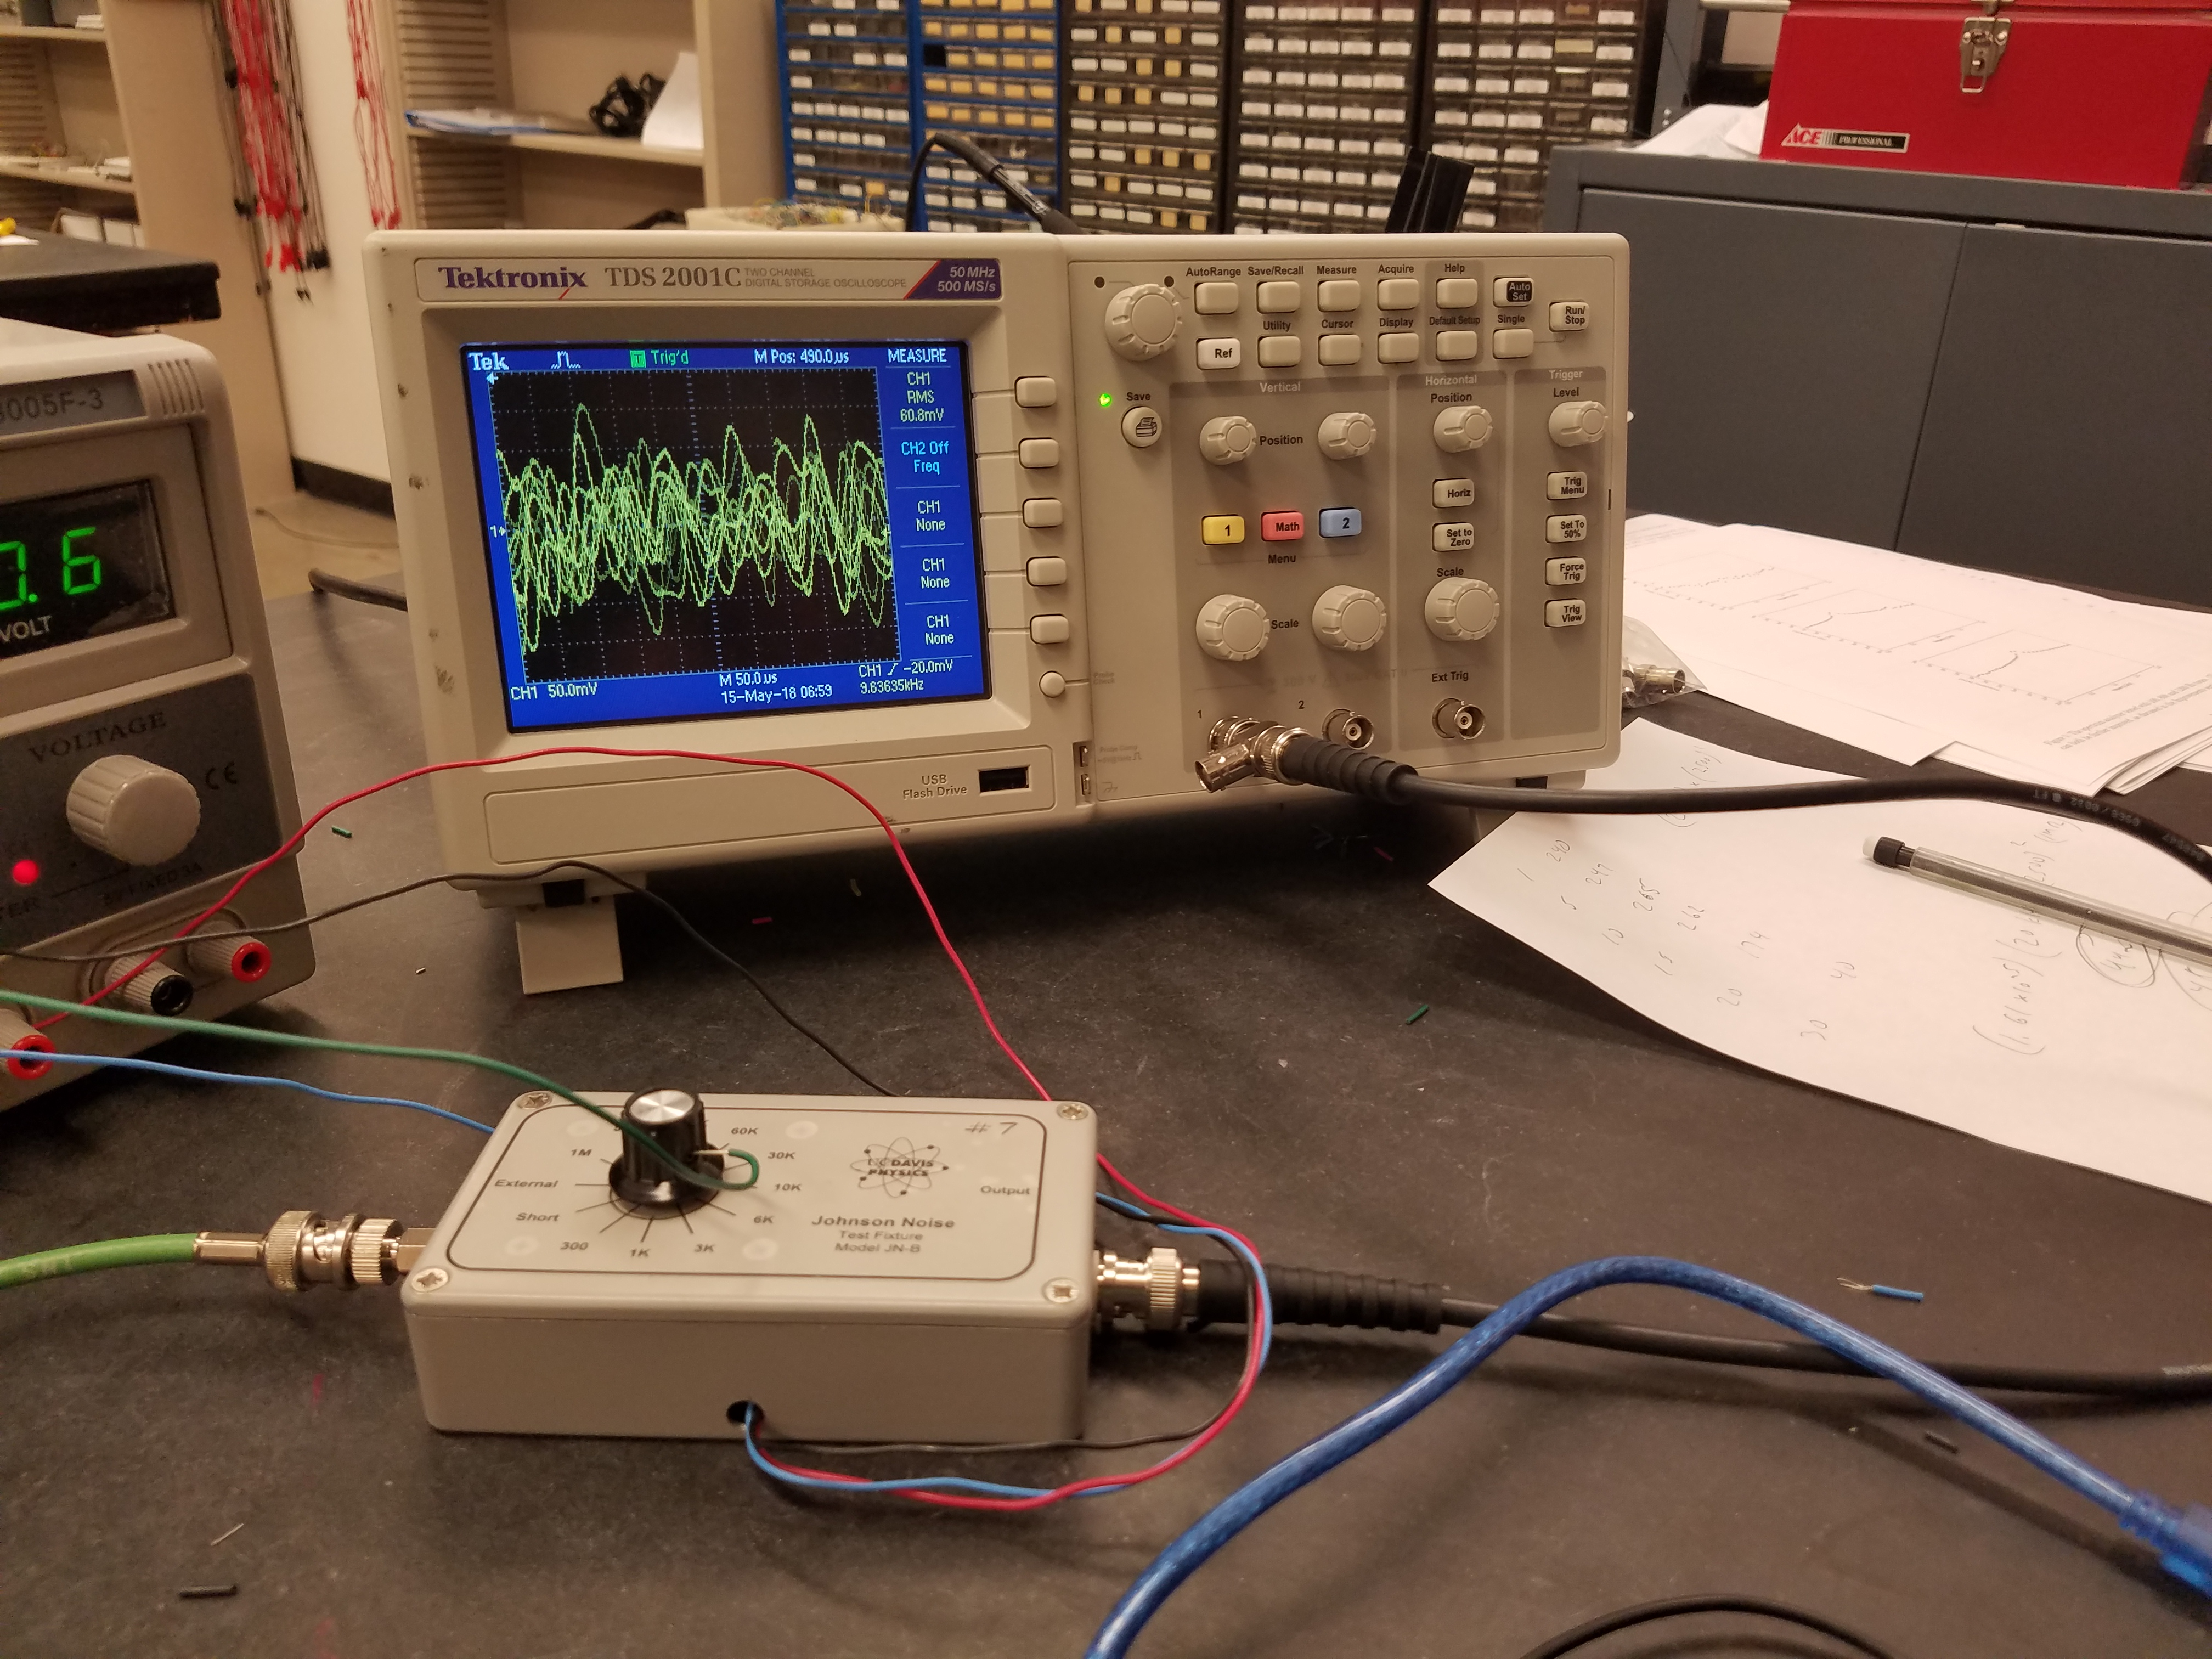
\includegraphics[width=0.65\textwidth]{figs/antenna_grounded.jpg}}
\end{center}
\caption{\label{fig:plan} Connections to the Johnson Noise device.  Note the grounding wire used to reduce noise from the knob acting as an antenna!}
\end{figure}

In this section, we will measure the gain of the Johnson Noise device as function of frequency.

Obtain a Johnson Noise (JN) measurement device (Model JN-A or JN-B) and note the serial number (e.g. \#4).  These are high gain devices that are very susceptible to damage.  Do not drive them directly from a function generator, but use a 1000:1 attenuator, taking care that the small resistor is toward the JN device (else you will reduce voltage by a factor 999/1000, and likely damage the equipment!)  

The JN devices are very sensitive, easily pickup noise, and ring at a characteristic frequency of about $27~{\rm kHz}$.  The tuning knob in particular picks up noise.  An old version banana plug cable plugged into the knob at the set screw grounds the knob, eliminated this source of noise.  The effect can be quite dramatic. 

Adjust the supply levels on your bench-top supply to $+12~{\rm V}$ and $-12~{\rm V}$.  Then, with the supply turned off, connect the JN device to power and ground, as labeled on the wires.  Once connected, power the device on and adjust the current thresholds to just slightly above where the supplies become current limited.  Under normal operation, the JN device should draw about $20~\rm mA$ from each supply... keep an eye on it.  If one of the supplies is inadvertently disconnected, the circuit latches in a high current state, which should be avoided if possible.

Set your function generator to produce a sine wave with $V_{\rm rms} = 1~\rm V$ and $f = 1~\rm kHz$.  
Connect the function generator to channel 1 of your scope, then to the $1000:1$ attenuator, and then to your JN device.  Make certain that the JN device is set to the ``External'' mode.  The output of the JN device should then be plugged directly into the scope channel 2.  This configuration puts significantly larger voltage at the JN device than a typical Johnson Noise signal.  Fortunately, the devices are quite linear, and this additional voltage will help overcome some sources of noise.

\begin{figure}[htbp]
\begin{center}
{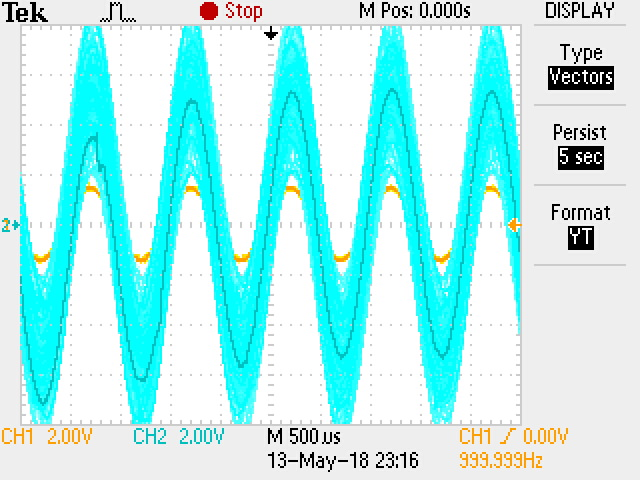
\includegraphics[width=0.65\textwidth]{figs/gaintrouble.jpg}}
\end{center}
\caption{\label{fig:gaintrouble} The output of the Johnson Noise device bounces around a lot due to low frequency noise.  Here the output is shown with display persistance.}
\end{figure}

Make a series of gain measurements at different frequencies that will allow to determine the integral
\begin{displaymath}
\int_{-\infty}^{\infty} df g(f)^2.
\end{displaymath}
While making the gain measurement, you will see that the output of the Johnson Noise seems to bounce around.  The effect can be seen if Fig.~\ref{fig:gaintrouble}.  There is a significant amount of low frequency noise in the output.  I found the best approach was to trigger on the AC line, which allows you to find a region of the plot with relatively little 60 Hz noise.  Use the scopes Measure capability to find the RMS voltage of the input and output of the Johnson Noise.  This is likely the major systematic uncertainty in your measurement, so spend some time thinking about how to quantify it. 

You might be tempted to try and use your DMM to measure the RMS voltage of your signal, but this is a mistake.  Your DMM is designed to measure 60~\rm Hz AC.

\section{Johnson Noise Measurement}
You are now ready to make your first-pass Johnson Noise measurement:
\begin{itemize}
\item Turn down the function generator and disconnect it from the JN device.

\item Turn the knob to select a resistor, and note the RMS voltage from the scope.  Repeat this measurement for every resistance.  
\end{itemize}

These measurements, combined with the gain measurement, should allow you to calculate $\kb$.
Before leaving, do make certain that the data you have collected is reasonable.  At this stage, within an order of magnitude of $\kb$ is acceptable.  {\bf This is the end point for week one.}  

\section{The Periodogram}

Suppose $V(t)$ is continuous with some period $T$ so that it is represented by a Fourier Series:
\begin{displaymath}
V(t) = \sum_{n=-\infty}^{\infty} c_n \exp(i2\pi f_n t)
\end{displaymath}
where $f_n = n / T$.  The Fourier coefficients are determined from:
\begin{equation}
c_n = \frac{1}{T} \int_{-\frac{T}{2}}^{\frac{T}{2}} dt \; V(t) \exp(-i2\pi f_n t), \label{eqn:freqcoeff}
\end{equation}
and in this context Parseval's theorem is:
\begin{displaymath}
\frac{1}{T} \int_{-\frac{T}{2}}^{\frac{T}{2}} |V(t)|^2 = \sum_n |c_n|^2
\end{displaymath}
or equivalently:
\begin{displaymath}
P_{\rm avg} \equiv \braket{|V(t)|^2} = \sum_n |c_n|^2
\end{displaymath}
which we can interpret to mean that $|c_n|^2$ represents the average power $P_{\rm avg}^{(n)}$ at frequency $f_n$.  Since the frequencies associated with each coefficient are discrete values separated by $\Delta f = f_{n+1} - f_{n} = 1/T $, the power spectral distribution for the discrete Fourier Series is
\begin{displaymath}
\mathcal{S}(f_n) = \frac{P_{\rm avg}^{(n)}}{\Delta f} = T |c_n|^2.
\end{displaymath}
Furthermore, since we often do not care about the {\em phase} information in the two-sided power spectral distribution, that is, we don't care to distinguish between power at $f_n$ and power at $-f_n$, the one-sided power spectral distribution is:
\begin{equation}
\mathcal{S}_{+}(f_n) = \frac{P_{\rm avg}^{(n)}}{\Delta f} = T (|c_n|^2 + |c_{-n}|^2) \label{eqn:discretepsd}
\end{equation}
It is left as an exercise to show that for
\begin{displaymath}
f(t) = A \cos( 2 \pi f_n t)
\end{displaymath}
the one-sided power spectral distribution is:
\begin{equation}
\mathcal{S}_{+}(f_n) = \frac{T}{2} |A|^2 \label{eqn:psdcalib}
\end{equation}
which is absolutely essential for calibrating a PSD using a function generator!

%
% Note also:  A_rms = sqrt(S/T) in keeping with S = V_rms^2 / dF
%

\begin{figure}[thb]
\begin{center}
{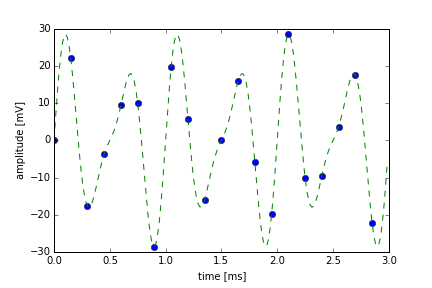
\includegraphics[width=0.55\textwidth]{figs/periodogram_ts.png}}\\
{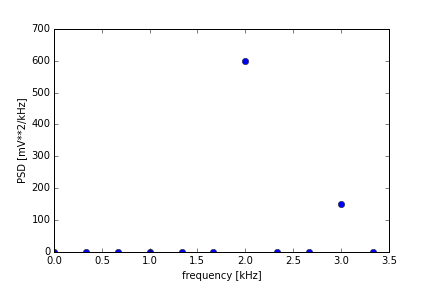
\includegraphics[width=0.55\textwidth]{figs/periodogram_eg.png}}
\end{center}
\caption{\label{fig:periodogram}  An example periodogram calculated from 20 samples over $3~\rm ms$ from a signal composed of two sine waves with amplitudes $10~\rm mV$ and $20~\rm mV$.  There are two peaks in the periodogram with PSD values $\mathcal{S}_{+}(f_n) = 150$ and $600~{\rm mV^2} / {\rm kHz}$ as expected from Equation~\ref{eqn:psdcalib}.
}
\end{figure}

In many cases, we wish to estimate the PSD from a discrete data set.  Instead of a continuous function of time $f(t)$ on the interval $T$ we instead have $N$ samples of $f$ each separated by time $\tau = T/N$, which we record as $x_i$.  We can replace $f(t)$ with its discrete version:
\begin{equation}
f(t) \to \sum_{m=0}^{N-1} x_m \; \delta(t - i\tau) \; \tau \label{eqn:discretef}
\end{equation}
so chosen because any integral over the discrete version
\begin{displaymath}
\int_{t_1}^{t_2} dt \sum_{m=0}^{N-1} x_m \; \delta(t - i\tau) \; \tau = \sum_{m=m_1}^{m_2} x_m  \tau
\to \int_{t_1}^{t_2} dt f(t)  
\end{displaymath}
approaches the integral over the continuous function in the limit $N \to \infty$.  Note that $m$ in the middle sum runs over the indices of the samples in the time interval $t_1$ to $t_2$.

Simply inserting the discrete version of $f(t)$ from Equation~\ref{eqn:discretef} into the formula for determining the coefficients of the Fourier series Equation~\ref{eqn:freqcoeff}:
\begin{eqnarray}
c_n &=& \frac{1}{T} \int_{-\frac{T}{2}}^{\frac{T}{2}} dt \; V(t) \exp(-i2\pi f_n t) \nonumber \\
&=& \frac{1}{T} \int_{-\frac{T}{2}}^{\frac{T}{2}} dt \; \exp\left(\frac{-i2\pi n t}{T} \right) \sum_{m=0}^{N-1} x_m\; 
\delta(t - i\tau) \; \tau \nonumber \\
&=& \frac{\tau}{T}  \sum_{m=0}^{N-1} \exp\left(\frac{-i2\pi n m \tau }{T} \right)  x_m \nonumber \\
&=& \frac{1}{N}  \sum_{m=0}^{N-1} \exp\left(\frac{-i2\pi n m }{N} \right)  x_m \label{eqn:dft}
\end{eqnarray}
This is an example of a discrete Fourier Transform (DFT).  There are more computationally efficient methods to calculate the coefficients $c_n$, but they all reproduce this calculation.  

The Nyquist-Shannon sampling theorem states that if the highest frequency component of a signal is $f_0$, and the signal is sampled at a rate $1/\tau \geq 2f_0$ then no information is lost.  The Fourier coefficients determined from the DFT can be used to exactly reproduce the original signal at any time.  This may seem surprising at first glance.  But consider that we are already familiar with a continous function being exactly represented by a discrete set of Fourier coefficients.  If a signal has a maximum frequency component $f_0$, we can think of it's Fourier transform as a periodic function on the interval $(-f_0, f_0)$.  It's inverse Fourier transform will then be discrete!

Given N samples $x_i$ taken at sample rate $1/\tau$, we calculate the DFT as the coefficients in Equation~\ref{eqn:dft}, then we calculate the one-sided power spectrum distribution as in Equation~\ref{eqn:discretepsd}.  If we have satisfied the Nyquist-Shannon sampling theorem, only the coefficients corresponding to $1/2\tau$ will be non-zero, so we need only report $\mathcal{S}_{+}(f_n)$ at the $N/2$ values from $f=1/T$ to $f=N/2T=1/2\tau$.  The plot of $\mathcal{S}_{+}(f_n)$ versus $f_n$ for these $N/2$ values is known as periodogram, and is a staple of digital signal processing.  An example periodogram resulting from a sine wave is shown in Fig.~\ref{fig:periodogram}.

Our initial assumption was that the function was periodic with time $T$, but often we apply periodograms to non-periodic signals, or signals with unknown periodicity.  In this case, there is a resolution loss if $1/T$.  This effect is mitigated by making $T$ as large as is feasible. 

\section{Digital Dynamic Range Adjustment}

In the second week of the lab, you will build a digital spectrum analyzer based on the Arduino Uno.
The Arduino's analog inputs have an input voltage range from 0 to 5 V, but our signals are ground referenced (symmetric about $0~\rm V$).  A DC level shifter is therefore needed to map the ground referenced output of the Johnson Noise device to the $0$ to $5~\rm V$ range expected by the Arduino analog inputs.  

Of course we'll be running the ADC as fast as possible which comes at the price of reduced resolution to 8 bits.  That would result in a voltage precision of $5~\rm V/ 2^8 \sim 20~\rm mV$.  Considering we will be looking at $\sim 100~\rm mV$ signals, this is just not enough precision.  Fortunately, we have one last trick up our sleeve!  The ADC has an (optional) external voltage reference, which sets the scale used by the ADC.  Experimentation showed that the ADC works reliably down to a voltage reference of $\sim 780~\rm mV$, which, at 8-bit precision, would give us a $3~\rm mv$ voltage precision, plenty good enough!

The low-pass filter in Fig.~\ref{fig:pwmfilt} is used to convert PWM output (on pin 5 of the Arduino) into a DC reference voltage $V_{\rm ref}$.  This reference voltage is used as (1) the reference for the ADC, at pin AREF, setting the dynamic range of the ADC, and (2) the reference to the DC level shifter circuit in Fig.~\ref{fig:offset} so that input to the ADC is referenced to $V_{\rm ref}/2$.  In this way, we can adjust $V_{\rm ref}$ to match the dynamic range of our signal, and the DC offset will be set to the middle of this range.  This will ensure that even for small signals, the full 8-bit precision of the ADC is being put to use.

\begin{figure}[htbp]
\begin{center}
\begin{circuitikz}[line width=1pt]
\draw (0,0) node[ground]{} to[pC,l=$C_1$,/tikz/circuitikz/bipoles/length=0.6cm] ++(0,1.5) coordinate(X);
\draw (X) to[R,l=$R_5$] ++(0,1.5) to[short,-o] ++ (-1.0,0) node[left]{$(5) \to V_{\rm pwm}$};
\draw (X) to[short,*-o] ++(1.0,0) node[right]{$V_{\rm ref} \to ({\rm AREF}) $};
\end{circuitikz} 
\end{center}
\caption{\label{fig:pwmfilt} A low pass filter used to convert the Arduino PWM output (on pin 5) to an analog DC reference voltage (sent to pin AREF and also used by the DC level shifter.)}
\end{figure}

\begin{figure}[htbp]
\begin{center}
\begin{circuitikz}[line width=1pt]
\draw (0,0) node[op amp, yscale=-1](opamp){}; 
\draw (opamp.-) to[short] ++(0.0,-1.0) coordinate(X) to[short] ++(1.0,0) to[R,l=$R_4$] ++(1.0,0) -| (opamp.out);
\draw (opamp.out) to[short,-o] ++(0.5,0) node[right]{$V_{\rm out} \to \rm (A0)$};
\draw (X) to[R,l_=$R_3$] ++(-1.5,0) node[ground]{};
\draw (opamp.+) to[short] ++(0,0.5) to[R,l_=$R_1$] ++(-1.5,0) to[short,-o] ++(0,0) node[left]{$V_{\rm in}$};
\draw (opamp.+) to[short] ++(0,-0.5) to[R,l_=$R_2$] ++(-1.5,0) to[short,-o] ++(0,0) node[left]{$({\rm AREF}) \to V_{\rm ref} $};
\end{circuitikz} 
\end{center}
\caption{\label{fig:offset} A DC level-shifter with unit gain.  The points (AREF) and (A0) refer to the Arduino pins, which should be connected as shown.}
\end{figure}

\begin{figure}[htbp]
\begin{center}
{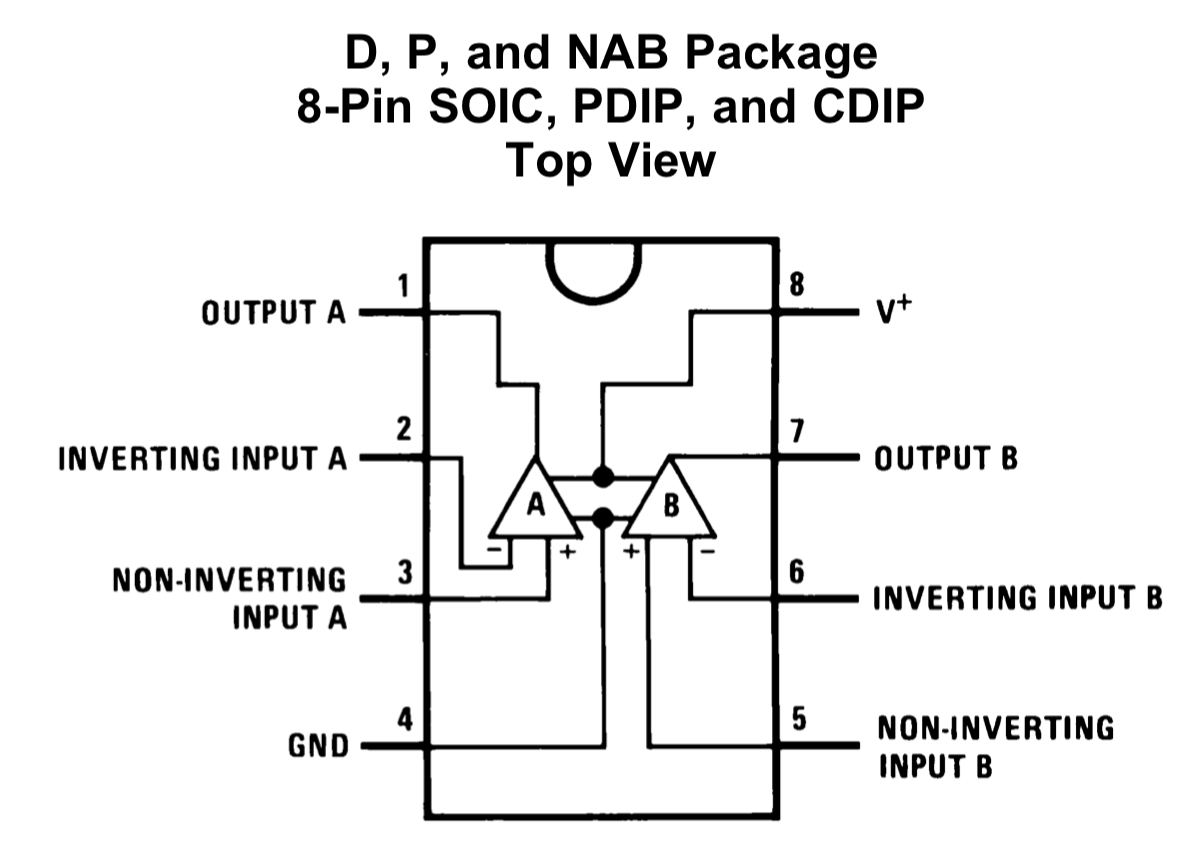
\includegraphics[width=0.65\textwidth]{figs/lm358.png}}
\end{center}
\caption{\label{fig:lm358} Pinout for the LM358 dual-op-amp with single-ended supply.  We'll only need one of the op-amps.}
\end{figure}

For our op-amp we will use a LM358 low-power dual op-amp IC with pinout in Fig.~\ref{fig:lm358}.
The LM358 is designed to run off a single supply down to $5~\rm V$, so we can power this circuit entirely from the Arduino.  This is not just convenient, it also ensures that it's output cannot exceed the $0$ to $5~\rm V$ range expected by the Arduino.

You will build the circuits in Fig.~\ref{fig:pwmfilt}  and \ref{fig:offset} using $R_1 = R_4 = 33~\rm k\Omega$, $R_2 = R_3 = 15~\rm k\Omega$, $R_5=1~k\Omega$.  For $C_1$ use a large polarized capacitor ($C_1=330~\rm  \mu F$) and {\bf make certain that the negative terminal is connected (as shown in the circuit) to ground.}  Connect the positive supply of the Op Amp to the $5~V$ supply of the Arduino and the $0~V$ supply to the Arduino ground.  

\begin{figure}[htbp]
\begin{center}
{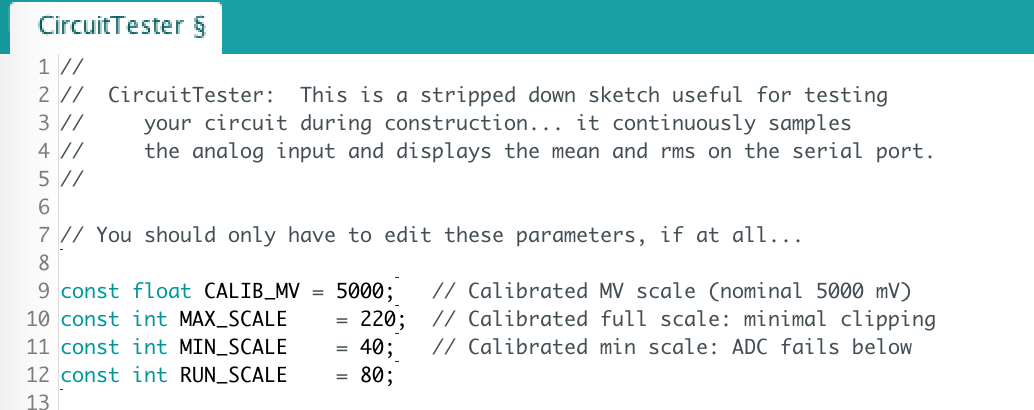
\includegraphics[width=0.45\textwidth]{figs/test_circuit.png}}\\
\end{center}
\caption{\label{fig:sketches}  The CircuitTester sketch is useful for developing, testing, and calibrating your circuit.  The sketch implements an RMS voltmeter that outputs directly to the Serial Monitor.  In the calibration section below you will calibrate CALIB\_MV which is set initially to the nominal $5~\rm V$ scale to match the actual full scale on your Arduino.  The scale refers to the PWM output which determines the reference voltage for the ADC.  A good all-around working point for this experiment is 80.}
\end{figure}

\begin{figure}[htbp]
\begin{center}
\begin{tabular}{cc}
{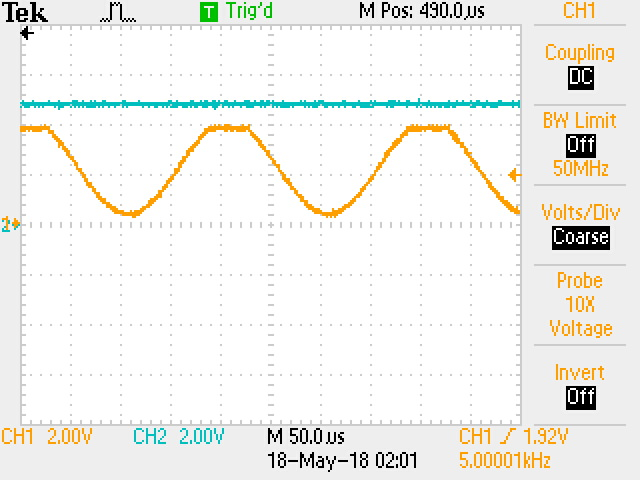
\includegraphics[width=0.45\textwidth]{figs/pwm255_1_3Vrms.JPG}} &
{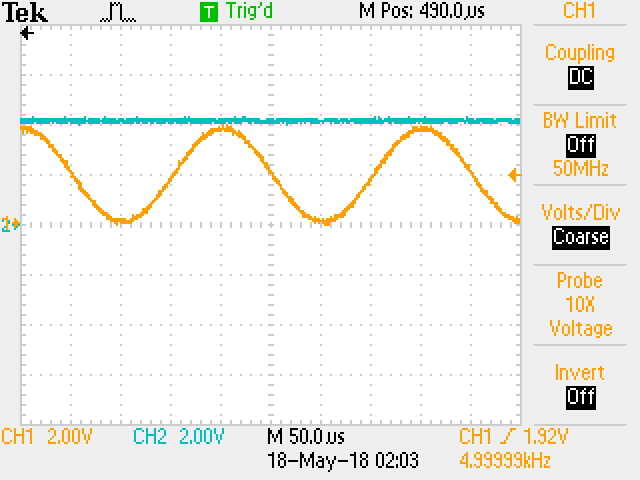
\includegraphics[width=0.45\textwidth]{figs/pwm220_1_3Vrms.JPG}} \\
(a) PWM=255, $V_{\rm rms}=1.3~\rm V$ & (b) PWM=220, $V_{\rm rms}=1.3~\rm V$ \\
{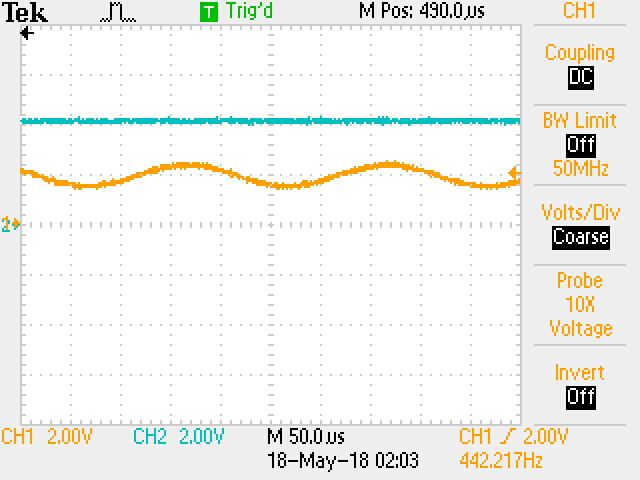
\includegraphics[width=0.45\textwidth]{figs/pwm220_300mVrms.JPG}} &
{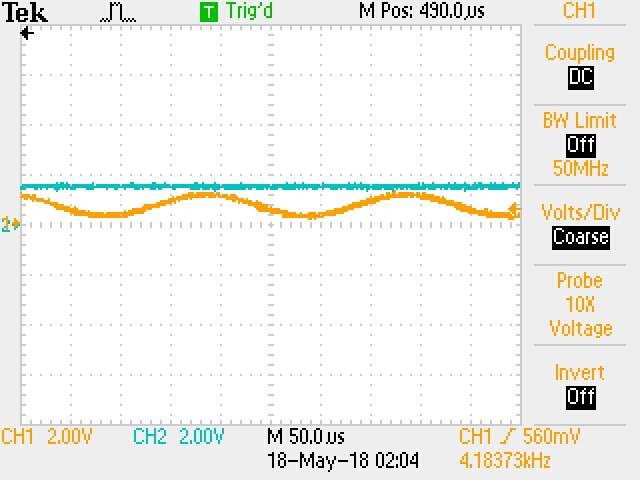
\includegraphics[width=0.45\textwidth]{figs/pwm80_300mVrms.JPG}} \\
(c) PWM=220, $V_{\rm rms}=300~\rm mV$ & (d) PWM=80, $V_{\rm rms}=300~\rm V$ \\
\end{tabular}
\end{center}
\caption{\label{fig:pwmdemo}  
Output of DC level-shifter compared to $V_{\rm ref}$ for various settings of the PWM analog output level
 and the function generator input RMS voltage.  In (a) the LM358 output does not reach the rail at 
 $5~\rm V$, so the ADC dynamic range above this cutoff is wasted.  In (b) the PWM setting at 220 adjusts $V_{\rm ref}$ to the full output range of the LM358, but (c) for low amplitude signals,
there is still wasted dynamic range.  In (d) the PWM setting at 80 matches the dynamic range of the signal.  Notice how the DC offset is automatically adjusted as well!
}
\end{figure}


A light-weight sketch {\rm CircuitTester} is provided which is useful while developing your circuit.  This sketch implements an RMS voltmeter (significantly better, if less durable, than the one provided by your DMM.) based on the circuit your are building.  It provides control of the PWM on pin 5, reads the analog input on A0, and regularly reports the RMS voltage (and other useful quantities) on the serial output.
The level of the PWM is specified in the parameter {\rm RUN\_SCALE}.  A value of 0 results in $0\%$ duty-cycle for the PWM, a value of 255 corresponds to $100\%$ duty-cycle.

While testing your circuit, you should use your function generator to drive the input $V_{\rm in}$ directly.  A $5~\rm kHz$ sine function with an RMS amplitude of $100~\rm mV$ is a good starting point.  Make sure the ground of the function generator is connected to the ground of your Arduino.

By now we've learned to divide and conquer technical challenges!  I'd propose something like:
\begin{itemize}
\item Leave the Arduino unpowered.
\item Build the level shifter as shown but at first (1) set the reference voltage to $5~\rm V$ and (2) connect the output to channel one on your scope instead of pin A0.
\item Power up the Arduino.
\item On your scope you should see the function generator referenced to approximately $2.5~\rm V$.
\item Power down the Arduino.
\item Build the lowpass filter as shown, but  connect $V_{\rm ref}$ to channel two on your scope instead of to pin {\tt AREF}.
\item Power up the Arduino and download the {\rm CircuitTester} sketch, setting the parameter {\tt RUN\_SCALE} to 112.
\item On your scope, you should observe $V_{\rm ref}$, it should be at about $2.5~\rm V$ with very little ripple (use AC line trigger and DC offset).
\item Adjust the {\tt RUN\_SCALE} parameter and ensure you have the expected behavior.
\item Power down the Arduino.
\item Connect the lowpass filter output $V_{\rm ref}$ to both $({\rm AREF})$ and the DC level-shifter input $V_{\rm ref}$.
\item Power up the Arduino.
\item Check that level-shifter output has the correct DC level when you adjust {\tt RUN\_SCALE}.
\item Connect the output of the DC level-shifter to the Arduino analog input A0.
\item Start the Serial Monitor.
\end{itemize}

Once the whole circuit is built, the Arduino is running the {\tt CircuitTester} sketch, and the Serial Monitor is open, you should observe periodic RMS voltage readings that should correspond approximately with the output of the function generator.  If it appears to be generally working but a bit inaccurate, you are ready for calibration.

\section{Calibration of Arduino Circuit}

An example of uncalibrated output from the CircuitTester sketch when connected to a $V_{\rm rms} = 300~\rm mV$ input signal is shown in Fig.~\ref{fig:uncalib}.   By design, the mean in raw ADC counts should be near $255/2$ within the accuracy of out $10\%$ resistors.  But the calibrated output in millivolts will be systematic off to start.  To calibrate, simply note the discrepancy and scale the CALIB\_MV parameter accordingly.  Once calibrated, you should get accurate measurements across a range of frequencies, amplitudes, and even $RUN_SCALE$ settings, as shown in Fig.~\ref{fig:calib}.  Take note of the value of CALIB\_MV as you will need to use it in the PSD python driver as well.

\begin{figure}[htbp]
\begin{center}
{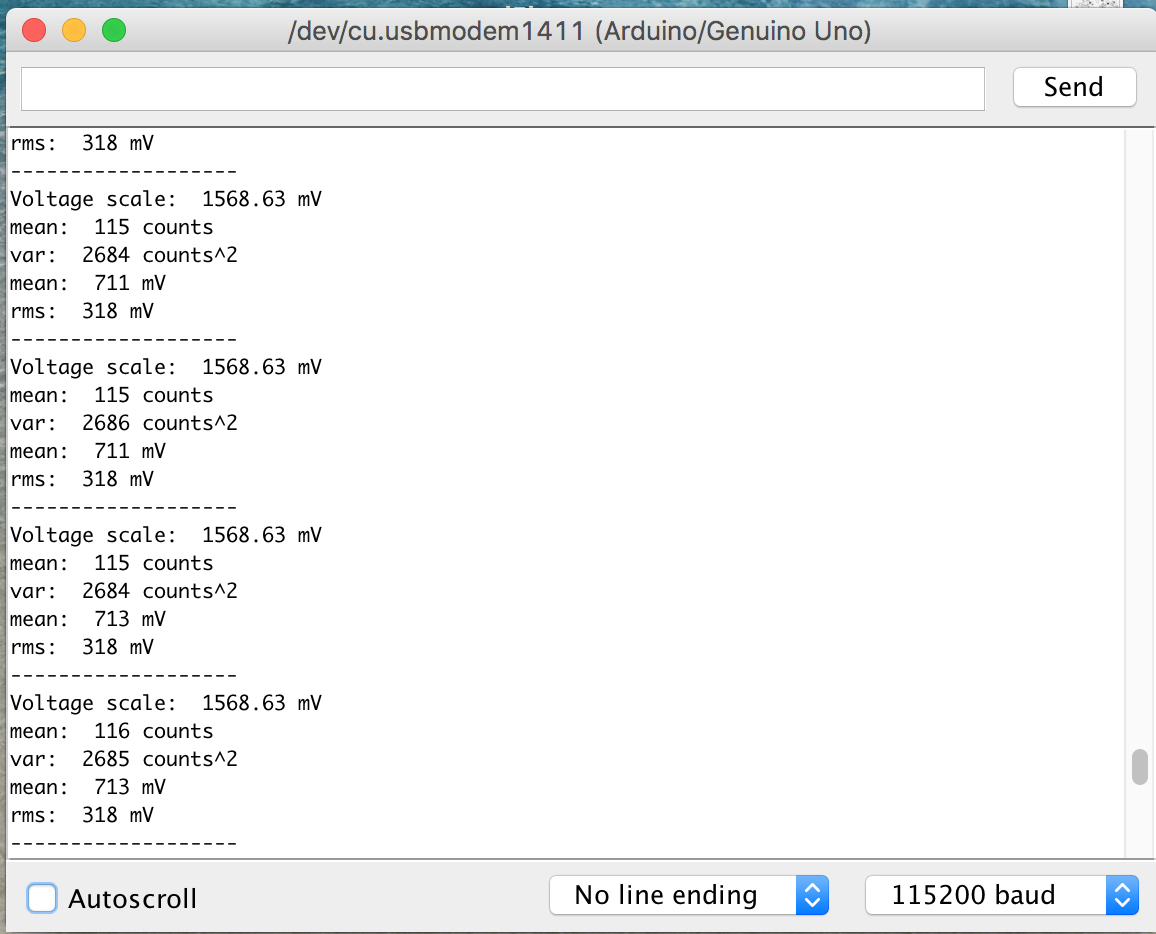
\includegraphics[width=0.65\textwidth]{figs/uncalibrated.png}}
\end{center}
\caption{\label{fig:uncalib} Uncalibrated Serial Monitor output for an input signal with $V_{\rm rms} = 300~\rm mV$.   It is systematically off at $318~\rm mV$ due to full scale being different than nominal $5~\rm V$.  The calibration is made by changing the value of {\tt CALIB\_MV} from 5000 to something more appropriate.
The mean, in RAW counts, is right where it should be:  near 255/2.}
\end{figure}

\begin{figure}[htbp]
\begin{center}
\begin{tabular}{cccc}
{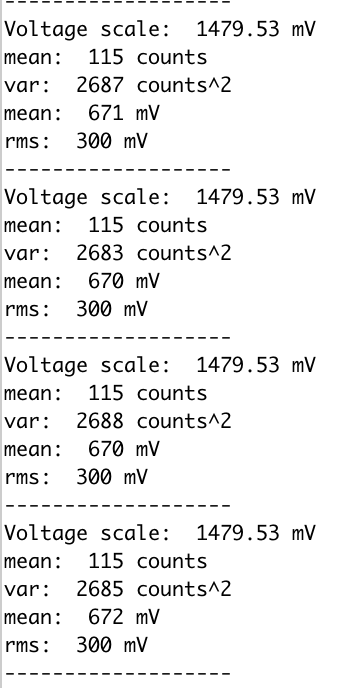
\includegraphics[height=0.30\textheight]{figs/caliba.png}} &
{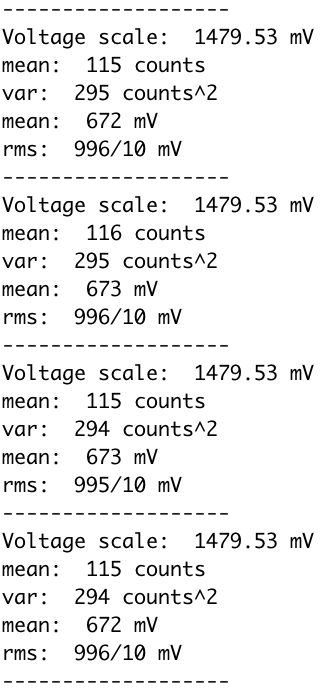
\includegraphics[height=0.30\textheight]{figs/calibb.png}} &
{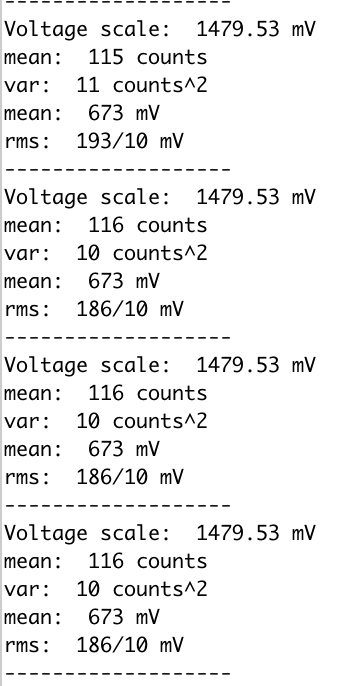
\includegraphics[height=0.30\textheight]{figs/calibc.png}} &
{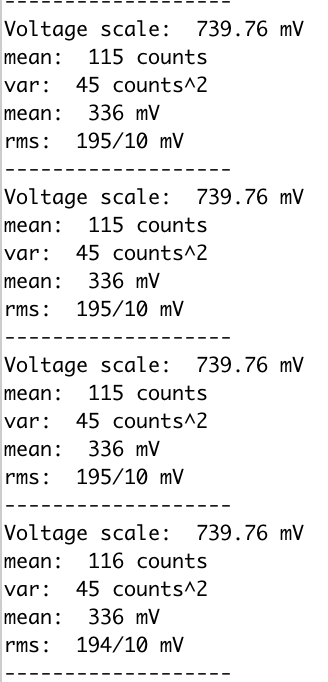
\includegraphics[height=0.30\textheight]{figs/calibd.png}} \\
(a) & (b) & (c) & (d) \\
\end{tabular}
\end{center}
\caption{\label{fig:calib}   Post-calibration output for an input signal with (a) $V_{\rm rms}=300~\rm mV$ (b) $V_{\rm rms}=100~\rm mV$ (c) $V_{\rm rms}=20~\rm mV$ (d) $V_{\rm rms}=20~\rm mV$.  In (a)-(c), the PWM analog output level is set to 80, a good choice for the gain calibration.  In (d) the range has been reduced to 40, resulting in better precision.  Also note that, for example, $186/10~\rm mV$ should be read as $18.6~\rm mV$... it seems {\tt sprintf} with float is not supported by the Arduino IDE.}
\end{figure}

\section{The Arduino Power Spectral Analyzer}

When your circuit is working and calibrated, you are ready to update the software to provide the Power Spectral Analyzer capability.  There is a new sketch (FastAdc) and a command line python driver (psd.py)
to provide this capability (see Fig.~\ref{fig:fastadc}.  The FastAdc sketch has the RUN\_SCALE parameter used to set the analog voltage scale, but the conversion to millivolts is done in the python driver, so you should set calib\_mv to the value your calibrated value.  As in the Fourier lab, if you tire of entering your COM port each time, you can hard code it in the driver.   Example output from running the python driver is shown in Fig.~\ref{fig:driver}.  As shown in Fig.~\ref{fig:response} the PSD performance is quite respectable, you can see this by scanning the frequency at a constant amplitude.  

Take the time to examine the output when the frequency goes above the Nyquist frequency (one half the sampling frequency, which is $39.8~\rm kHz$ in our case).  You should see clear aliasing of the high-frequency signal at a lower frequency.  Fortunately, the low-pass filter in the Johnson Noise device eliminates problematic high-frequency aliasing during our experiment.

\begin{figure}[htbp]
\begin{center}
{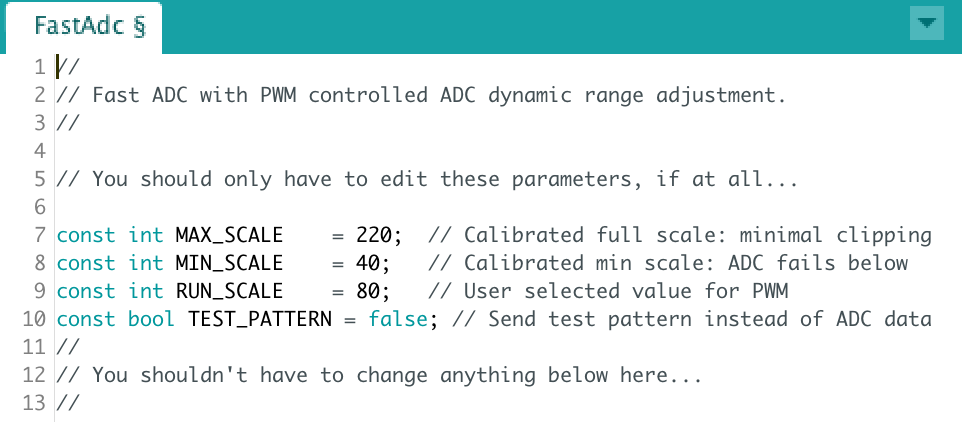
\includegraphics[width=0.45\textwidth]{figs/fast_adc.png}}
\end{center}
\caption{\label{fig:fastadc}    
The FastAdc sketch is used together with the psd.py python driver on your PC.  The sketch only uses raw adc counts, but the calibration calib\_mv in psd.py should match what you determine with CircuitTester.  
The PWM output which controls the analog voltage reference is controlled by the RUN\_SCALE parameter.
A good all-around working point for this experiment is 80.
}\end{figure}

\begin{figure}[htbp]
\begin{center}
{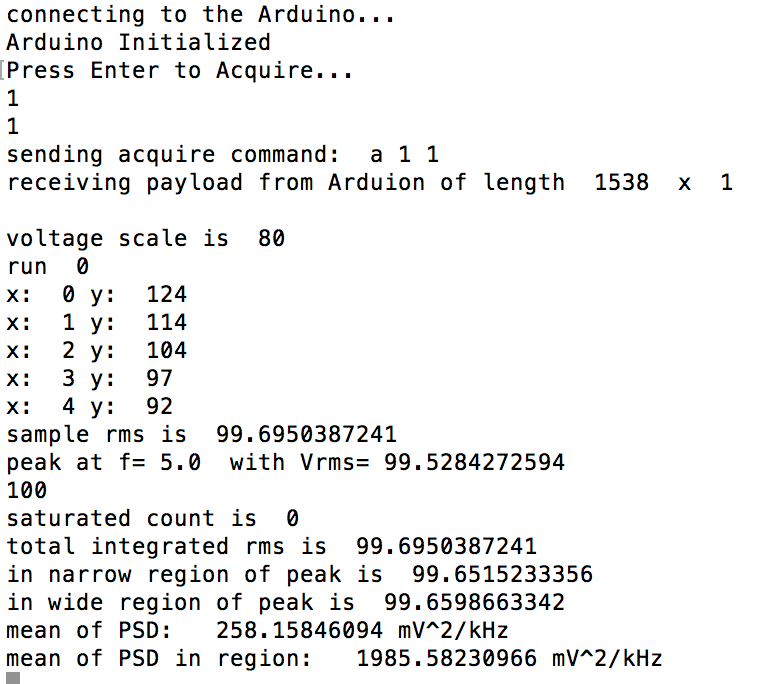
\includegraphics[width=0.65\textwidth]{figs/psd_driver.png}}\\
{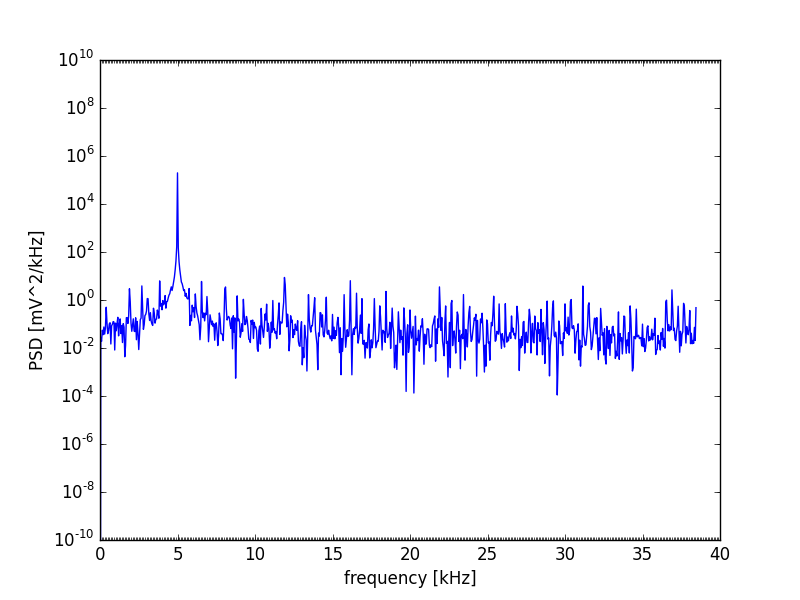
\includegraphics[width=0.65\textwidth]{figs/psd_5k.png}}
\end{center}
\caption{\label{fig:driver}  The python serial driver psd.py as seen at the command line (top) and the (bottom) power spectral distribution plot it produces.  This output is for an input with $V_{\rm rms} = 100~\rm mV$ and $f=5~\rm kHz$.
}\end{figure}

\begin{figure}[htbp]
\begin{center}
{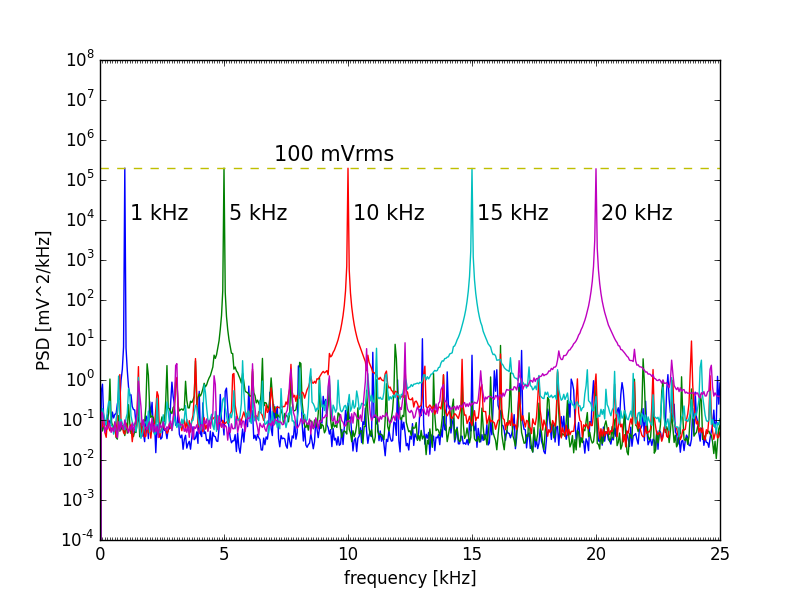
\includegraphics[width=0.65\textwidth]{figs/response.png}}
\end{center}
\caption{\label{fig:response}  The response of the Arduino PSD.}\end{figure}

\section{Improved Johnson Noise Device Gain Measurement}

The scope gain measurement is quite imprecise due to the presence of significant (few volts) low-frequency noise whenever the function generator is connected to the JN device.  This noise is unambiguously due to an unavoidable (with your available test equipment) small ground loop between the function generator and your bench-top DC power supply.  The tiny amount of noise due to this ground loop is amplified by the JN device by a factor of 1000.  High gain instruments are a challenge!  

By moving this analysis into frequency space, we can largely avoid the low frequency noise in our measurement.  Using your Arduino spectrum analyzer, collect data for a range of frequencies, as shown in Fig.~\ref{fig:gain_raw}.  You should use the nruns parameter in the python sketch to average 10 runs per measurement (default is one run only), reducing statistical fluctuations in your power spectrum.  You will use these samples to determine the gain of the JN device as function of frequency.  The python driver always saves the data it collected from the Arduino to the file "data.npy".  You'll simply have to rename this file to something else for each sample you collect, before taking the next sample.  Example python for plotting the data saved in such a file is included on the course website (plot.py). 

\begin{figure}[htbp]
\begin{center}
{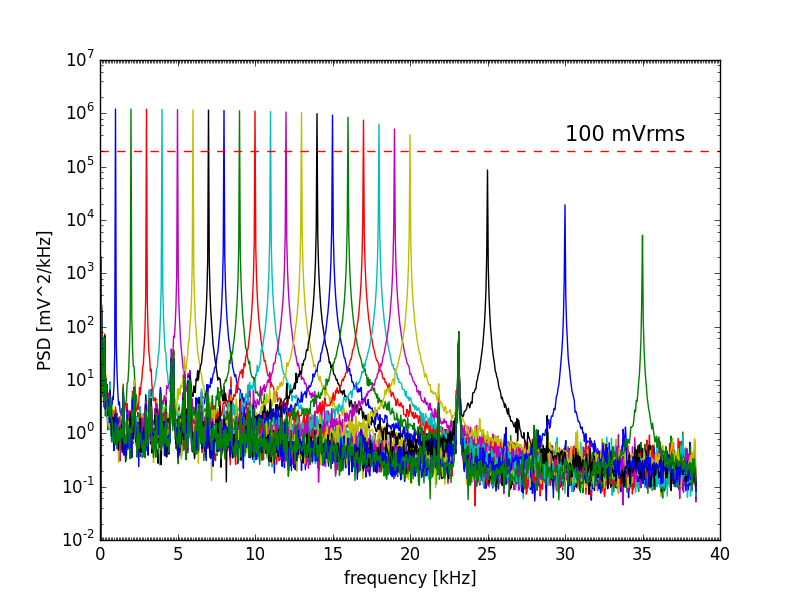
\includegraphics[width=0.65\textwidth]{figs/gain_raw.png}}
\end{center}
\caption{\label{fig:gain_raw}  Data collected for gain versus frequency scan.}\end{figure}

Unfortunately, the ground loop noise is not completely overcome by the power spectral analysis.   The noise is so large that it saturates the ADC during some portion of the sample collection, effectively filtering out the higher frequency signal of interest, and systematically reducing our gain estimate.

\begin{table}[htbp]
\begin{center}
\begin{tabular}{lll}
Device & $5~\rm kHz$ & $10~\rm kHz$ \\ 
JN-A-\#6 & 3.77 & 3.49 \\
JN-A-\#1 & 3.82 & 3.51 \\
JN-A-\#3 & 3.83 & 3.60 \\
JN-A-\#3 & 3.86 & 3.61 \\
JN-A-\#2 & 3.85 & 3.55 \\
JN-B-\#9 & 2.47 & 2.39 \\
JN-B-\#7 & 2.57 & 2.75 \\
\end{tabular}
\end{center}
\caption{\label{tbl:gain} Measured gain for each device at two benchmark frequencies.   These gains are accurate to better than $5\%$.}
\end{table}

Using an isolating transformer to break the ground loop by floating the function generator ground effectively eliminates this noise.  Each JN device has been calibrated using this technique, and the measured gains at $5~\rm kHz$ and $10~\rm kHz$ are recorded in Table~\ref{tbl:gain}.  The shape of your gain as a function of frequency can be inferred reliably from your data, but your should apply an overall scale factor to match one of the benchmarks at the benchmark frequency.  This will give you a reliable Gain curve, accurate to about $5\%$.

\section{Johnson Noise Measurement}

With your instrument calibrated, you are ready to collect Johnson noise data
You should attempt to demonstrate at least the following three things:
\begin{itemize}
\item The flat frequency spectrum of Johnson Noise.
\item The linear relation between Johnson Noise and the resistance. 
\item An experimental measurement of $\kb$, including an uncertainty.
\end{itemize}
With a bit of luck (and an isolation transformer!) I was able to measure $\kb$ to within 1\% of it's value (See Fig.~\ref{fig:noise}).

\begin{figure}[htbp]
\begin{center}
{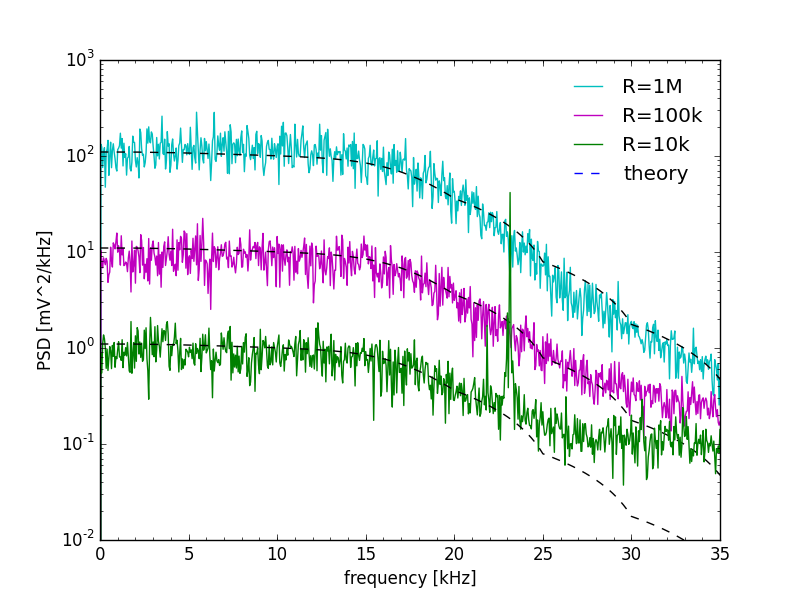
\includegraphics[width=0.65\textwidth]{figs/compare_psd.png}}
\end{center}
\caption{\label{fig:compare_psd}  Example data collected for Johnson Noise measurement, compared to the expectation including the measured gain.}\end{figure}

\begin{figure}[htbp]
\begin{center}
{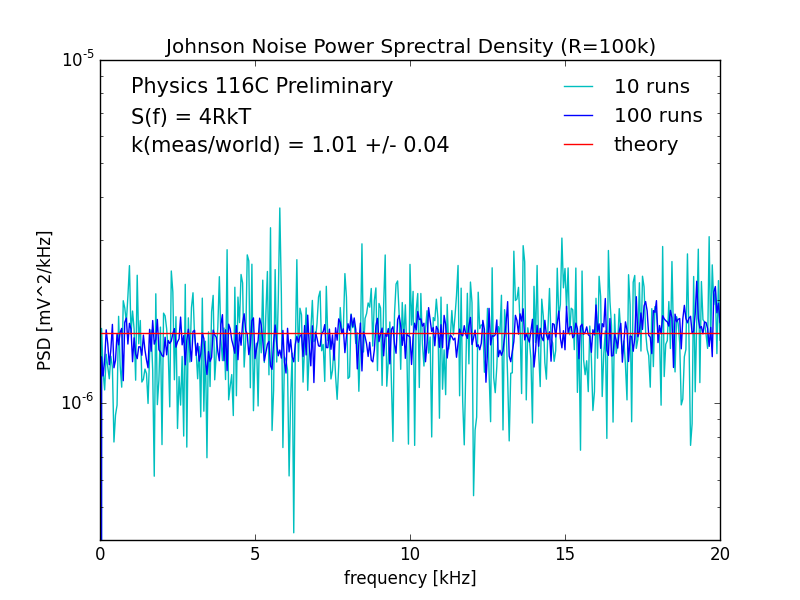
\includegraphics[width=0.65\textwidth]{figs/noise.png}}
\end{center}
\caption{\label{fig:noise}  Not bad! }\end{figure}

\end{document}


